%\documentclass[spanish]{beamer}

\documentclass{beamer}
\usepackage{pgf,pgfpages}
%\pgfpagesuselayout{4 on 1}[letterpaper,landscape,border shrink=0.5in]
\usepackage{algorithm,algorithmic}
%\usepackage{algorithm,algorithmicx}
%\usepackage[noend]{algpseudocode}
\usepackage{listings}
\lstset{basicstyle=\ttfamily,
	showstringspaces=false,
	commentstyle=\color{red},
	literate={á}{{\'a}}1
	{ã}{{\~a}}1
	{é}{{\'e}}1
	{É}{{\'E}}1
	{ó}{{\'o}}1
	{í}{{\'i}}1
	{ñ}{{\~n}}1
	{¡}{{!`}}1
	{¿}{{?`}}1
	{ú}{{\'u}}1
	{Í}{{\'I}}1
	{Ó}{{\'O}}1
}

\usepackage{beamerthemesplit}
\usepackage{color}
\usepackage[utf8]{inputenc}
\usepackage[spanish]{babel}
%\usepackage[latin1]{inputenc}
%\usepackage[pdftex]{graphicx}
%\usepackage{algorithm}
%\usepackage{algorithmic-C}
%\usepackage{algorithmic}
\usepackage{amsthm}
\usepackage{multicol}
\usepackage{multirow}
\usepackage{fancyvrb,relsize}
\usepackage{hhline}
\usepackage{tikz}
\usetikzlibrary{trees, shapes, calc}
\newcommand{\inputTikZ}[2]{%
	\scalebox{#1}{\input{#2}}
}

\usetheme{Warsaw} %Gueno
%\usetheme{Darmstadt} %OK!
% \usetheme{Frankfurt} %OK!
%\usetheme{Goettingen}
%\usetheme{Dresden}
%\usetheme{JuanLesPins} %OK!!
%\usetheme{Marburg}
%\usetheme{Montpellier}
%\usetheme{Rochester} %sobrio
%\usetheme{Singapore}
%\usetheme{Szeged}

%\usecolortheme{albatross}
%\usecolortheme{seahorse}
%\usecolortheme{beetle}
%\usecolortheme{crane}
%\usecolortheme{dolphin}
%\usecolortheme{dove}
%\usecolortheme{fly}
%\usecolortheme{lily} %Gueno
\usecolortheme{orchid}%Gueno
%\usecolortheme{rose}
%\usecolortheme{seagull}
%\usecolortheme{whale}


\DefineVerbatimEnvironment%
      {VerbatimNN}%
      {Verbatim}%
      {fontsize=\relsize{-1}}
\DefineVerbatimEnvironment%
      {VerbatimNNN}%
      {Verbatim}%
      {fontsize=\relsize{-2}}

\DefineVerbatimEnvironment%
      {VerbatimPseudo}%
      {Verbatim}%
      {numbers=left, fontsize=\relsize{-1}}
\DefineVerbatimEnvironment%
      {VerbatimPseudoReduced}%
      {Verbatim}%
      {numbers=left, fontsize=\relsize{-2}}
\DefineVerbatimEnvironment%
      {VerbatimPseudoReduced2}%
      {Verbatim}%
      {numbers=left, fontsize=\relsize{-3}}
\DefineVerbatimEnvironment%
      {VerbatimC}%
      {Verbatim}%
      {commandchars=@ªº, numbers=left, fontsize=\relsize{-1}}
\DefineVerbatimEnvironment%
      {VerbatimReducedC}%
      {Verbatim}%
      {commandchars=@ªº, numbers=left, fontsize=\relsize{-2}}
\DefineVerbatimEnvironment%
      {VerbatimReduced2C}%
      {Verbatim}%
      {commandchars=@ªº, numbers=left, fontsize=\relsize{-3}}



%\AtBeginSubsection[]
%{
% \begin{frame}
% \frametitle{Sinopsis}
% Aqui decides: cada seccion y subseccion:
% \tableofcontents[currentsection,currentsubsection]
 %O solamente la seccion (Solo uno de ellos)
%\tableofcontents[currentsection]
% \end{frame}
%}

% Si quieres que todo por default aparezca de poco en poco
% descomenta esta linea
%\beamerdefaultoverlayspecification{<+->}

\setbeamertemplate{footline}{\hfill\insertframenumber/\inserttotalframenumber}
\setbeamertemplate{navigation symbols}{}

\setbeamercovered{transparent}

\title{ELO320 - Estructuras de Datos y Algoritmos\\Introducción a C\\Memoria Dinámica}
%\subtitle{Ingeniería Civil Telemática UTFSM}
\author{Dr. Nicolás Gálvez R.\\{\small nicolas.galvez@usm.cl}}
\institute{Ing. Civil Telemática - Departamento de Electrónica}
\titlegraphic{
\includegraphics[scale=.18]{images/logoutfsm}}
\date{2do Semestre 2022}

\begin{document}

\frame{\titlepage}

%\section*{Sinopsis}
%\frame{  \frametitle{Sinopsis}\tableofcontents[pausesections]}
%
%

\section{Memoria dinámica.}
\begin{frame}[fragile]{Memoria dinámica.}

La memoria dinámica es aquella que cae bajo control del programador y se almacena el \textbf{heap} de la memoria. 

Es un elemento necesario porque:
\begin{itemize}
\item Los arreglos fijos son espacios de memoria contigua cuyo tamaño no es modificable.
\item ¿Qué pasa si definimos un tamaño y es insuficiente?
\item ¿Qué pasa si el arreglo reserva más memoria que su uso real?
\end{itemize}
\end{frame}

\begin{frame}[fragile]{Memoria dinámica.}
\begin{itemize}
\item Memoria Dinámica: Se reserva memoria en el heap. 
\item Se accede a esta memoria mediante punteros.
\item 3 instrucciones básicas de \texttt{stdlib.h}:
\begin{itemize}
\item \texttt{malloc()}: reserva de memoria.
\item \texttt{realloc()}: reasignación de memoria.
\item \texttt{free()}: liberación de memoria.
\end{itemize}
\item \texttt{valgrind}: software para debugging de temas relacionados con memoria.
\end{itemize}
\end{frame}

\begin{frame}[fragile]{Memoria dinámica: \texttt{malloc}}
\begin{itemize}
\item Instrucción para la reserva de memoria.
\item Entrega como resultado la dirección de memoria donda inicia la reserva.
\item \textbf{Necesitamos punteros}.
\item Operador \texttt{sizeof} como base del tamaño a reservar. 
\begin{exampleblock}{C}
\begin{lstlisting}[language=C, basicstyle=\tiny, escapeinside={|}{|}]
#include<stdio.h>
#include<stdlib.h>

int main(int argc, char **argv){
	int *arreglo=NULL;

	arreglo = malloc(10 * sizeof(*arreglo));
//	arreglo = malloc(10 * sizeof(int));
//	arreglo = malloc(10 * sizeof *arreglo); 

	// sizeof es un operador: sizeof(tipo_de_dato) o sizeof expresion
        // cast no es necesario, compilador hacecoerción.
	// solo para compatibilidad con C++, se usa
//	arreglo = (int *) malloc(10 * sizeof(int)); 
	return 0;
}
\end{lstlisting}
\end{exampleblock}
\end{itemize}
\end{frame}

\begin{frame}[fragile]{Memoria dinámica: \texttt{realloc}}
\begin{itemize}
\item Instrucción para la reasignar memoria ya reservada.
\item Si se agranda la memoria, esta puede cambiar completamente de dirección.
\begin{exampleblock}{C}
\begin{lstlisting}[language=C, basicstyle=\tiny, escapeinside={|}{|}]
#include<stdio.h>
#include<stdlib.h>

int main(int argc, char **argv){
	int *arreglo=NULL;

	arreglo = malloc(10 * sizeof(*arreglo));

	// libera 5 ints, mantiene dir.
	arreglo = realloc(arreglo, 5 * sizeof(int));

	// se expande en 15 ints, mantiene dir si existe
	// espacio contiguo, sino se cambia.
	arreglo= realloc(arreglo, 20 * sizeof * arreglo);

	return 0;
}
\end{lstlisting}
\end{exampleblock}
\end{itemize}
\end{frame}

\begin{frame}[fragile]{Memoria dinámica: \texttt{free}}
\begin{itemize}
\item Instrucción para liberar la memoria reservada en heap.
\item Los ejemplos anteriores no liberaban memoria.
\item Sirve para liberar los recursos ociosos y no cometer en el manejo (memory leaks).

\begin{exampleblock}{C}
\begin{lstlisting}[language=C, basicstyle=\tiny, escapeinside={|}{|}]
#include<stdio.h>
#include<stdlib.h>

int main(int argc, char **argv){
	int *arreglo=NULL;

	arreglo = malloc(10 * sizeof(*arreglo));

	// libera 5 ints, mantiene dir.
	arreglo = realloc(arreglo, 5 * sizeof(int));

	// se expande en 15 ints, mantiene dir si existe
	// espacio contiguo, sino se cambia.
	arreglo= realloc(arreglo, 20 * sizeof * arreglo);

	free(arreglo);
	return 0;
}
\end{lstlisting}
\end{exampleblock}
\end{itemize}
\end{frame}

\section{Problemas con punteros.}

\frame[containsverbatim]
{
\frametitle{Dangling}
\begin{itemize}
\item \textbf{Dejar Colgado (dangling).} 
\item Puntero hacia localización de memoria del heap que ha sido liberada (e incluso nuevamente asignada). 
\item Genera errores poco predecibles (e.g. Segmentation fault, corrupción de memoria).
\end{itemize}
\begin{exampleblock}{C}
\begin{lstlisting}[language=C, basicstyle=\tiny, escapeinside={|}{|}]
int main(int argc, char **argv){
	int x=2;
	int *p, *q;

	p= malloc(sizeof(int));
	q=p;

	free(p);  /* q aun mantiene referencia al heap */
        	 /* puede que variable de heap sea reasignada */

	*q = x;

	return 0;
}
\end{lstlisting}
\end{exampleblock}
}


\frame[containsverbatim]
{
\frametitle{Fuga de memoria - Memory Leak}
\begin{itemize}
\item \textbf{Fuga de memoria (memory leak)}. 
\item Pérdida de acceso a objeto de memoria reservado en el heap, por no existir variables que apunten a él. 
\item No se puede liberar hasta el término del programa.
\item Puede saturar la memoria.
\end{itemize}
\begin{exampleblock}{C}
\begin{lstlisting}[language=C, basicstyle=\tiny, escapeinside={|}{|}]
int main(int argc, char **argv){
	int *p;
	
	p= malloc(sizeof(int));
	p= malloc(sizeof(int));
	/* se pierde la direccion asignada anteriormente */

	free(p);

	return 0;
\end{lstlisting}
\end{exampleblock}
}

\frame[containsverbatim]
{
\frametitle{Ejemplo}

\begin{center}
{\centering \Large Dangling}
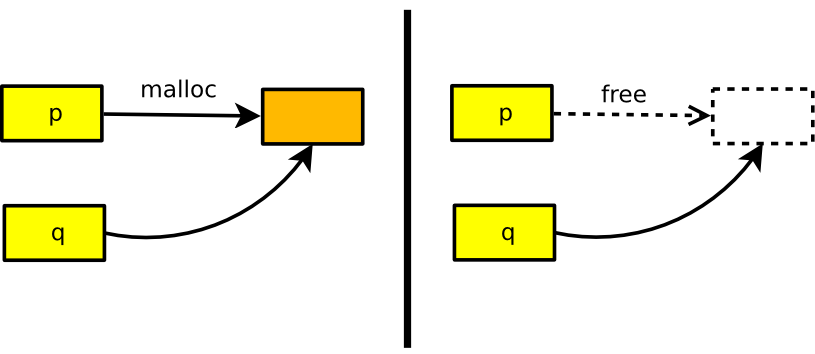
\includegraphics[width=.85\linewidth]{images/dangling}\\
{\centering \Large Memory Leak}
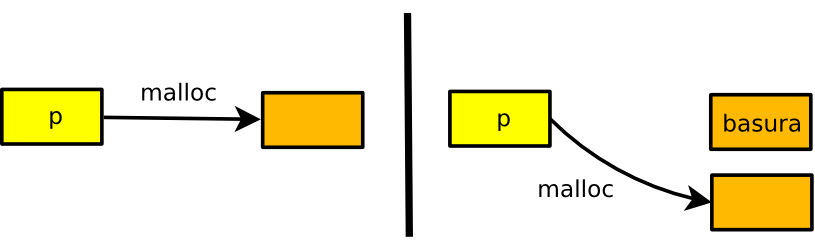
\includegraphics[width=.85\linewidth]{images/lostheap}
\end{center}
}

\begin{frame}[fragile]{Memoria dinámica: Ejemplo}
\begin{exampleblock}{C}
\begin{lstlisting}[language=C, basicstyle=\tiny, escapeinside={|}{|}]
#include<stdio.h>
#include<stdlib.h>

int main(int argc, char **argv){

	int *arreglo=NULL, i;

	arreglo = malloc(10 * sizeof *arreglo); // sizeof(int) o sizeof(*arreglo)
	// sizeof es un operador: sizeof(tipo_de_dato) o sizeof expresion
        // cast no necesario, coerción. solo para compatibilidad con C++.

	if(arreglo==NULL){
		printf("Error, memoria mal reservada...\n");
		return -1;
	}

	for(i=0;i<5;i++){
		arreglo[i]=i+1;
	}

	arreglo = realloc(arreglo, 5* sizeof(int)); //reducimos a 5 ints

	for(i=0;i<5;i++){
		printf("|\%|d ", arreglo[i]);
	}

	free(arreglo); //libera memoria 
	return 0;
}
\end{lstlisting}
\end{exampleblock}
\end{frame}

\frame[containsverbatim]
{
\frametitle{Memoria dinámica: Ejemplo}

\begin{center}
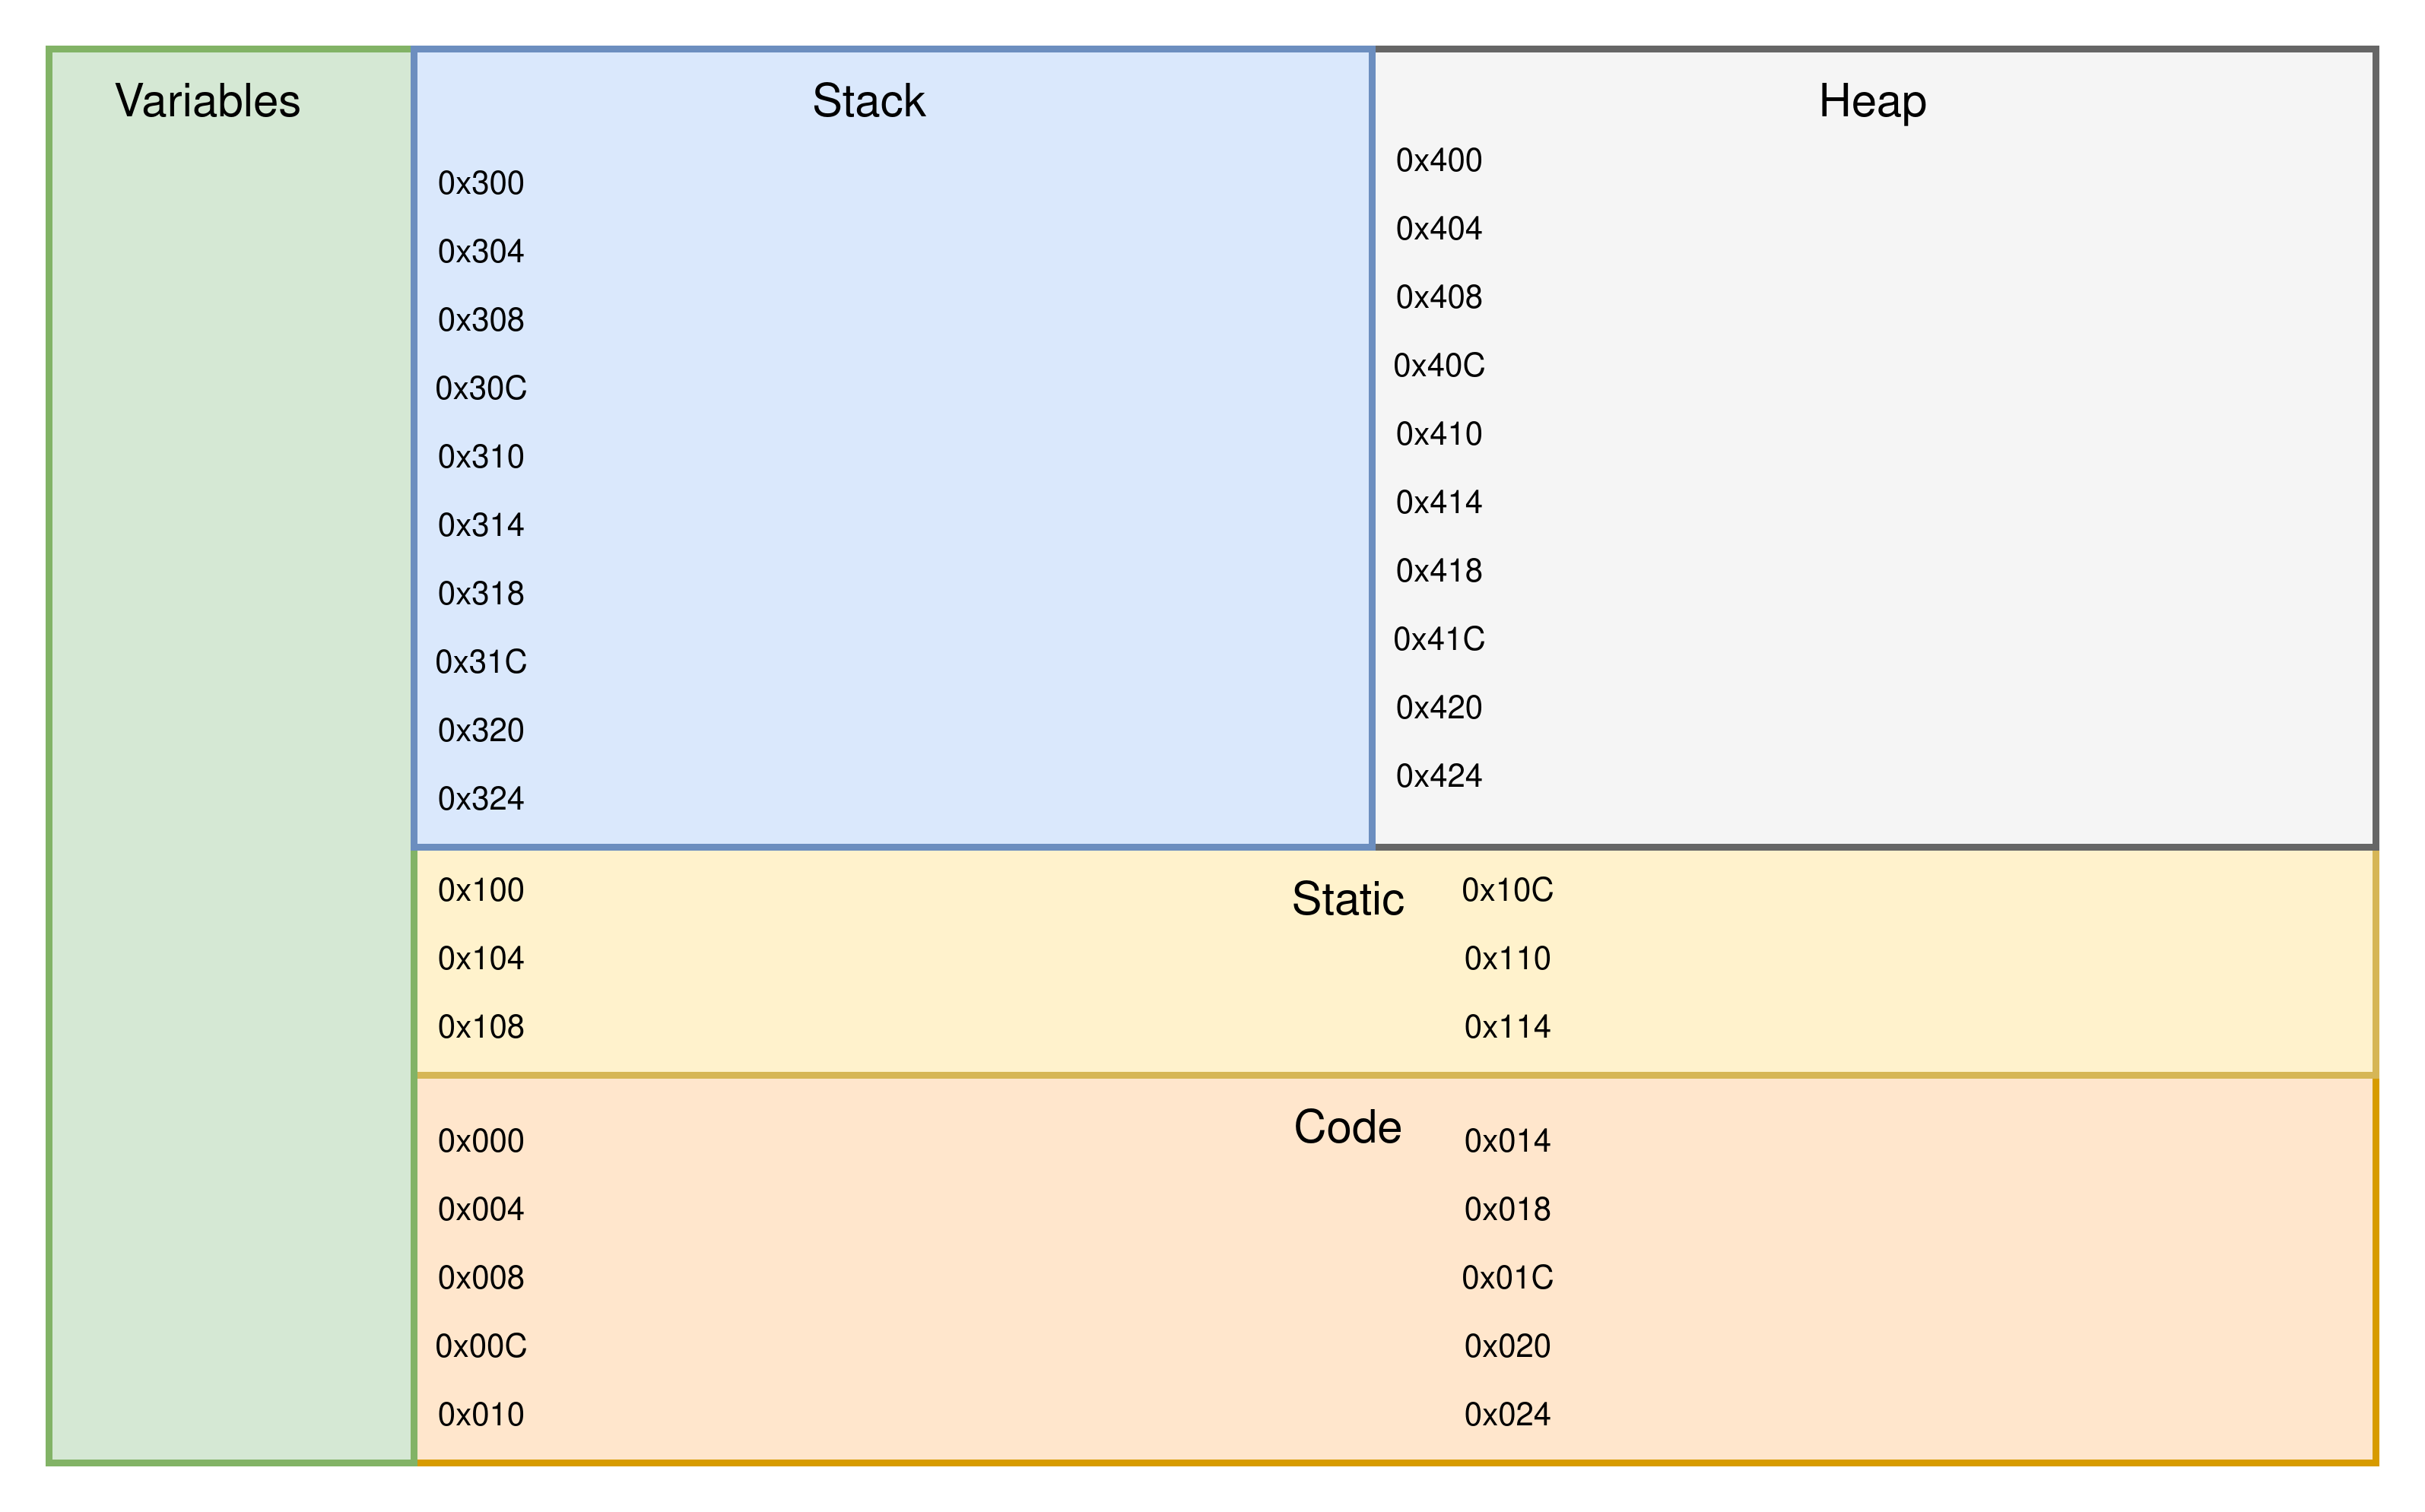
\includegraphics[width=\linewidth]{images/memoryscheme}
\end{center}
}





\end{document}
